\chapter{Research Statement}\label{chap:research_proposal}

This chapter will provide an overview of the problem this thesis is trying to solve. First, a brief description of MULTI-VP's workflow is provided (Section \ref{sec:multivp}), followed by existing methods for initial flow estimation (Section \ref{sec:ml_initial_flow}).  An extensive analysis of the data used in the previous and subsequent approaches is done in Section \ref{sec:data_analyis}. This thesis's hypothesis and research questions are proposed in Section \ref{sec:hypothesis}. 

\section{MULTI-VP}\label{sec:multivp}

MULTI-VP \cite{pinto.rouillard_MultipleFluxtubeSolar_2017} is a global MHD model that simulates the three-dimensional structures of the solar wind. In addition, it also estimates the conditions at the Sun's chromosphere, transition region, corona, and low heliosphere. The model computes many one-dimension solar wind solutions from full flux-tube geometries and heating functions. Background magnetic field geometries are extrapolated from publicly available magnetogram data. The method can estimate solar wind profiles across the Sun's atmosphere up to 30 solar radii. The results directly link the geometry of magnetic flux tubes in the lower corona with the distributions of fast and slow solar wind flows. MULTI-VP proved faster than other MHD models and did not suffer from cross-field diffusion effects. For a more in-depth data analysis, refer to the next chapter.

\vspace{0.5cm}
\begin{figure}[]
\centering
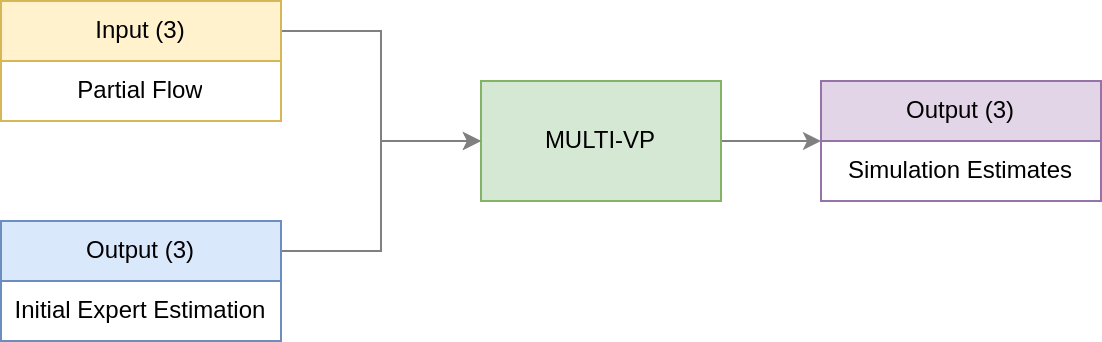
\includegraphics[width=0.8\textwidth]{figures/multivp_method.png}
\caption[MULTI-VP methodology dataflow]{MULTI-VP methodology dataflow. The model takes the partial flow and its associated expert initial guess as input and then derives a better solution.\label{fig:multivp_method}}
\end{figure}

A MULTI-VP simulation workflow overview can be seen in Figure \ref{fig:multivp_method}. It takes as input flux-tube partial flows and initial expert estimations for the solar wind conditions. After a long simulation time, these last estimations are approximated to final estimates more congruent with the actual conditions on the Sun's surface.




\section{ML for Initial Flow Estimation}\label{sec:ml_initial_flow}
Due to its complexity and many calculations, MULTI-VP, like other MHD simulations, still takes a long time to reach viable solar wind predictions. Furthermore, the need for initial expert guesses also significantly delays the process. These factors directly affect the prediction capability and preparation for extreme solar events. Recently in "Initial Condition Estimation in Flux Tube Simulations using Machine Learning" \cite{barros_InitialConditionEstimation_}, it has been proved that machine learning techniques can accurately produce good initial flow conditions that MULTI-VP can later use. The authors also proved that the quality of the flow estimations is directly linked to the total execution time of the simulation. These allow for faster convergence of the MHD simulation as the initial estimates are closer to the final solution. 

\begin{figure}[h]
\centering
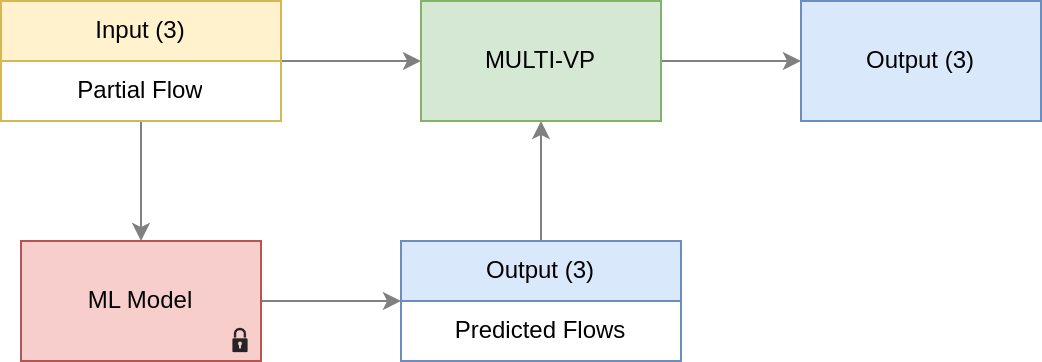
\includegraphics[width=0.8\textwidth]{figures/multivp_rnn.png}
\caption[ML methodology dataflow]{ML methodology dataflow. An ML model estimates the initial conditions of a given partial flow. These are then passed to MULTI-VP, approximating them into a final solution. \label{fig:multivp_rnn}}
\end{figure}

\begin{figure}[]
    \centering
    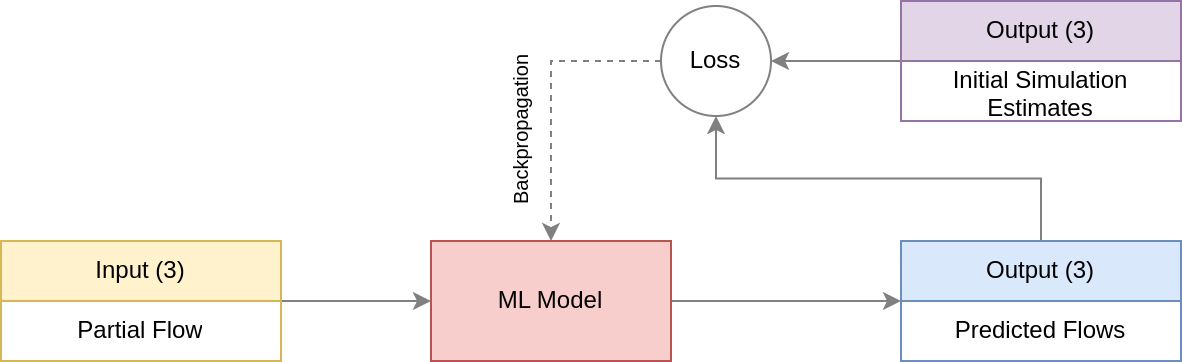
\includegraphics[width=0.8\textwidth]{figures/rnn_training.png}
    \caption[ML training phase]{Model training method. Takes as input initial partial flows and tries to predict flow estimates close to the ones from previous MULTI-VP simulations.\label{fig:rnn_train}}
\end{figure}

The approach, illustrated in Figure \ref{fig:multivp_rnn}, uses an ML model to predict the initial expert estimates from the initial partial flow input. Analogous to the method presented in Section \ref{sec:multivp}, MULTI-VP takes as input the partial flows along with their initial conditions predicted by the ML model.

An illustration of the training method can be seen in Figure \ref{fig:rnn_train}. In this phase, the model takes as inputs initial partial flows and tries to predict the initial conditions. Next, the predictions for a given flow are compared to those from previous MULTI-VP runs to calculate the prediction's loss and update the model's parameters with backpropagation. The logic behind this was that the model would learn to predict initial estimations closer to the final solution, and thus, the simulation would converge faster.

Due to the high simulation time of MULTI-VP, a small number of files were randomly selected from the whole dataset to be used as a validation set. These were excluded from the training and testing phases. The performance of the ML method was evaluated by feeding MULTI-VP with the predictions of the validation dataset and then assessing the error of the simulation estimates and the overall computation time.

However, the reduction in execution time was minimal. The authors posit that the presence of anomalies during the training phase might have hampered the overall prediction quality of the model. Another potential issue arises from the nature of the data, which exhibits significant dispersion, with high concentrations in certain areas and low concentrations in others. This characteristic can pose challenges as the neural network model tends to converge towards the densely populated points, potentially failing to learn the patterns in the peripheral areas.

\section{Exploratory Data Analysis}\label{sec:data_analyis}
The data used by MULTI-VP and the prediction model consists of magnetogram data from the Wilcox Solar Observatory. Each file contains 12 columns representing measurements of the magnetic field in the solar atmosphere at different heights. Every variable comprises 640 points (abscissas) measured at different radial distances from the Sun (up to 30 Solar radii). In addition, the data is distributed evenly throughout five batches, each consisting of solar wind measurements at different surface locations. For this work, only six columns will be used, as the others are derivations of these and, thus, are redundant. 

\begin{table}[h]
    \caption{Data columns of magnetogram used by MULTI-VP.}
    \label{tab:multivp_columns}
    \begin{subtable}[h]{0.32\textwidth}
        \centering
        \begin{tabular}{lcc}
        \hline
        \multicolumn{3}{c}{Input (Partial Flows)}                              \\ \hline
        $R${[}$R_{sun}${]} & $B${[}$G${]} & $\alpha${[}$deg${]} \\ \hline
        \end{tabular}
    \end{subtable}
    \begin{subtable}[h]{0.32\textwidth}
        \centering
        \begin{tabular}{ccc}
        \hline
        \multicolumn{3}{c}{Output (Estimations)}                           \\ \hline
        $n${[}$cm^{-3}${]} & $v${[}$km/s${]} & $T${[}$MK${]} \\ \hline
        \end{tabular}
    \end{subtable}
\end{table}

The data columns can be seen in Table \ref{tab:multivp_columns}. These are divided into two parts: the input and the output (predictions). The former comprises the set of variables the simulation uses to approximate solar wind conditions, and the latter the initial expert guesses needed to kickstart the multiple flux simulation. Note that, like in Barros \cite{barros_InitialConditionEstimation_} (Figure \ref{fig:rnn_train}), the output variables are the predictions of previous MULTI-VP simulations and not actual expert predictions.

The input data includes the magnetic field amplitude, $B$, the flux tube inclination, $\alpha$, and the radial coordinate, $R$. The output data consists of the number of charged particles per unit volume, $n$, the velocity, $v$, and the temperature, $T$.



Figure \ref{fig:jointplot_input} shows a joint plot of the input variables. Based on these plots, it can be inferred that several input files contain anomalous data. This is evident from the graph of variable B, where specific files exhibit significant deviations from the overall distribution. Furthermore, there are instances of faulty lines within the normal distribution, which further complicates the detection of these anomalies.


\begin{figure}
    \centering
    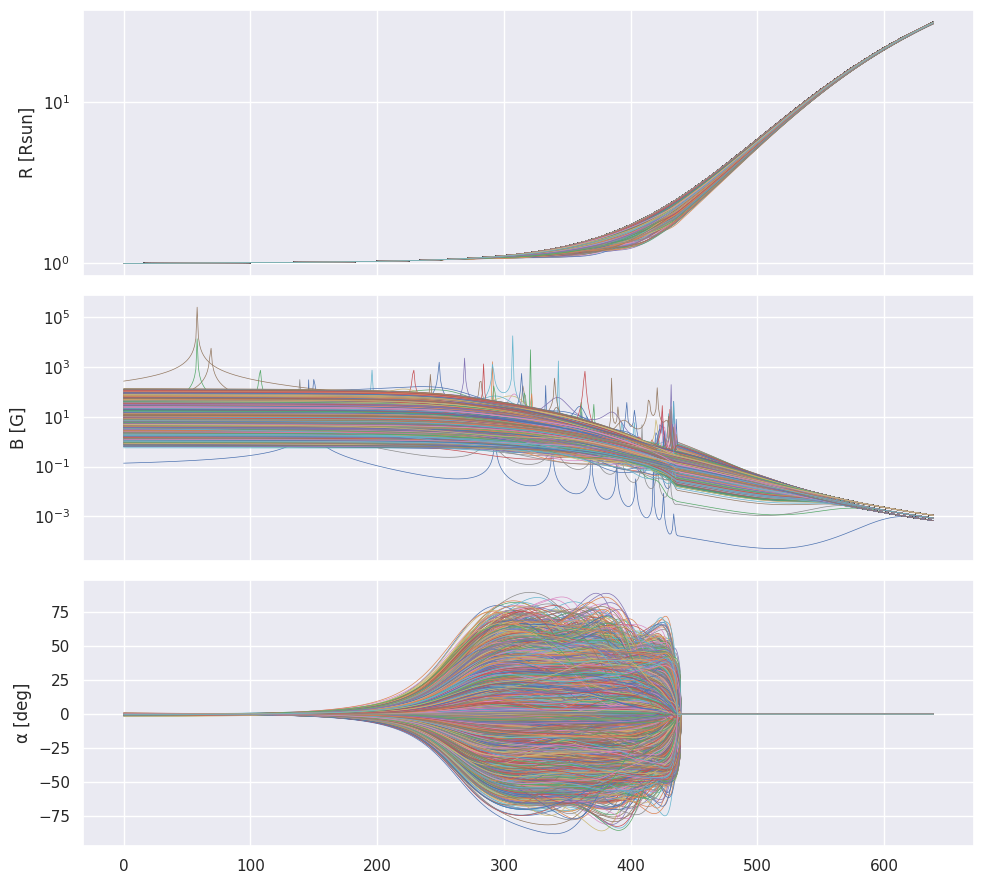
\includegraphics[width=0.8\textwidth]{figures/joint_input_cols.png}
    \caption[Joint plot of the inputs of MULTI-VP]{Joint plot of the input variables of each file used in this work. The first row is the plot of the radial coordinate radius, $R$, the second the magnetic field, $B$, and the last the flux tube inclination $\alpha$. All are plotted in function of position in the magnetogram file.}
    \label{fig:jointplot_input}
\end{figure}

As previously explained (in Section \ref{sec:multivp}), MULTI-VP requires initial expert guesses to kickstart the simulation. These consist of the output variables presented in Table \ref{tab:multivp_columns} and, during the simulation, are approximated to better solutions. In line with the work carried out in Barros \cite{barros_InitialConditionEstimation_}, we will be using the outputs of previous simulations as initial guesses (refer to Figure \ref{fig:rnn_train}) for more details). Figure \ref{fig:jointplot_output} shows the joint plot of the output variables. Similar to the input plots, several faulty predictions can be seen in all variable plots, resulting from simulations carried out on anomalous inputs.

\begin{figure}
    \centering
    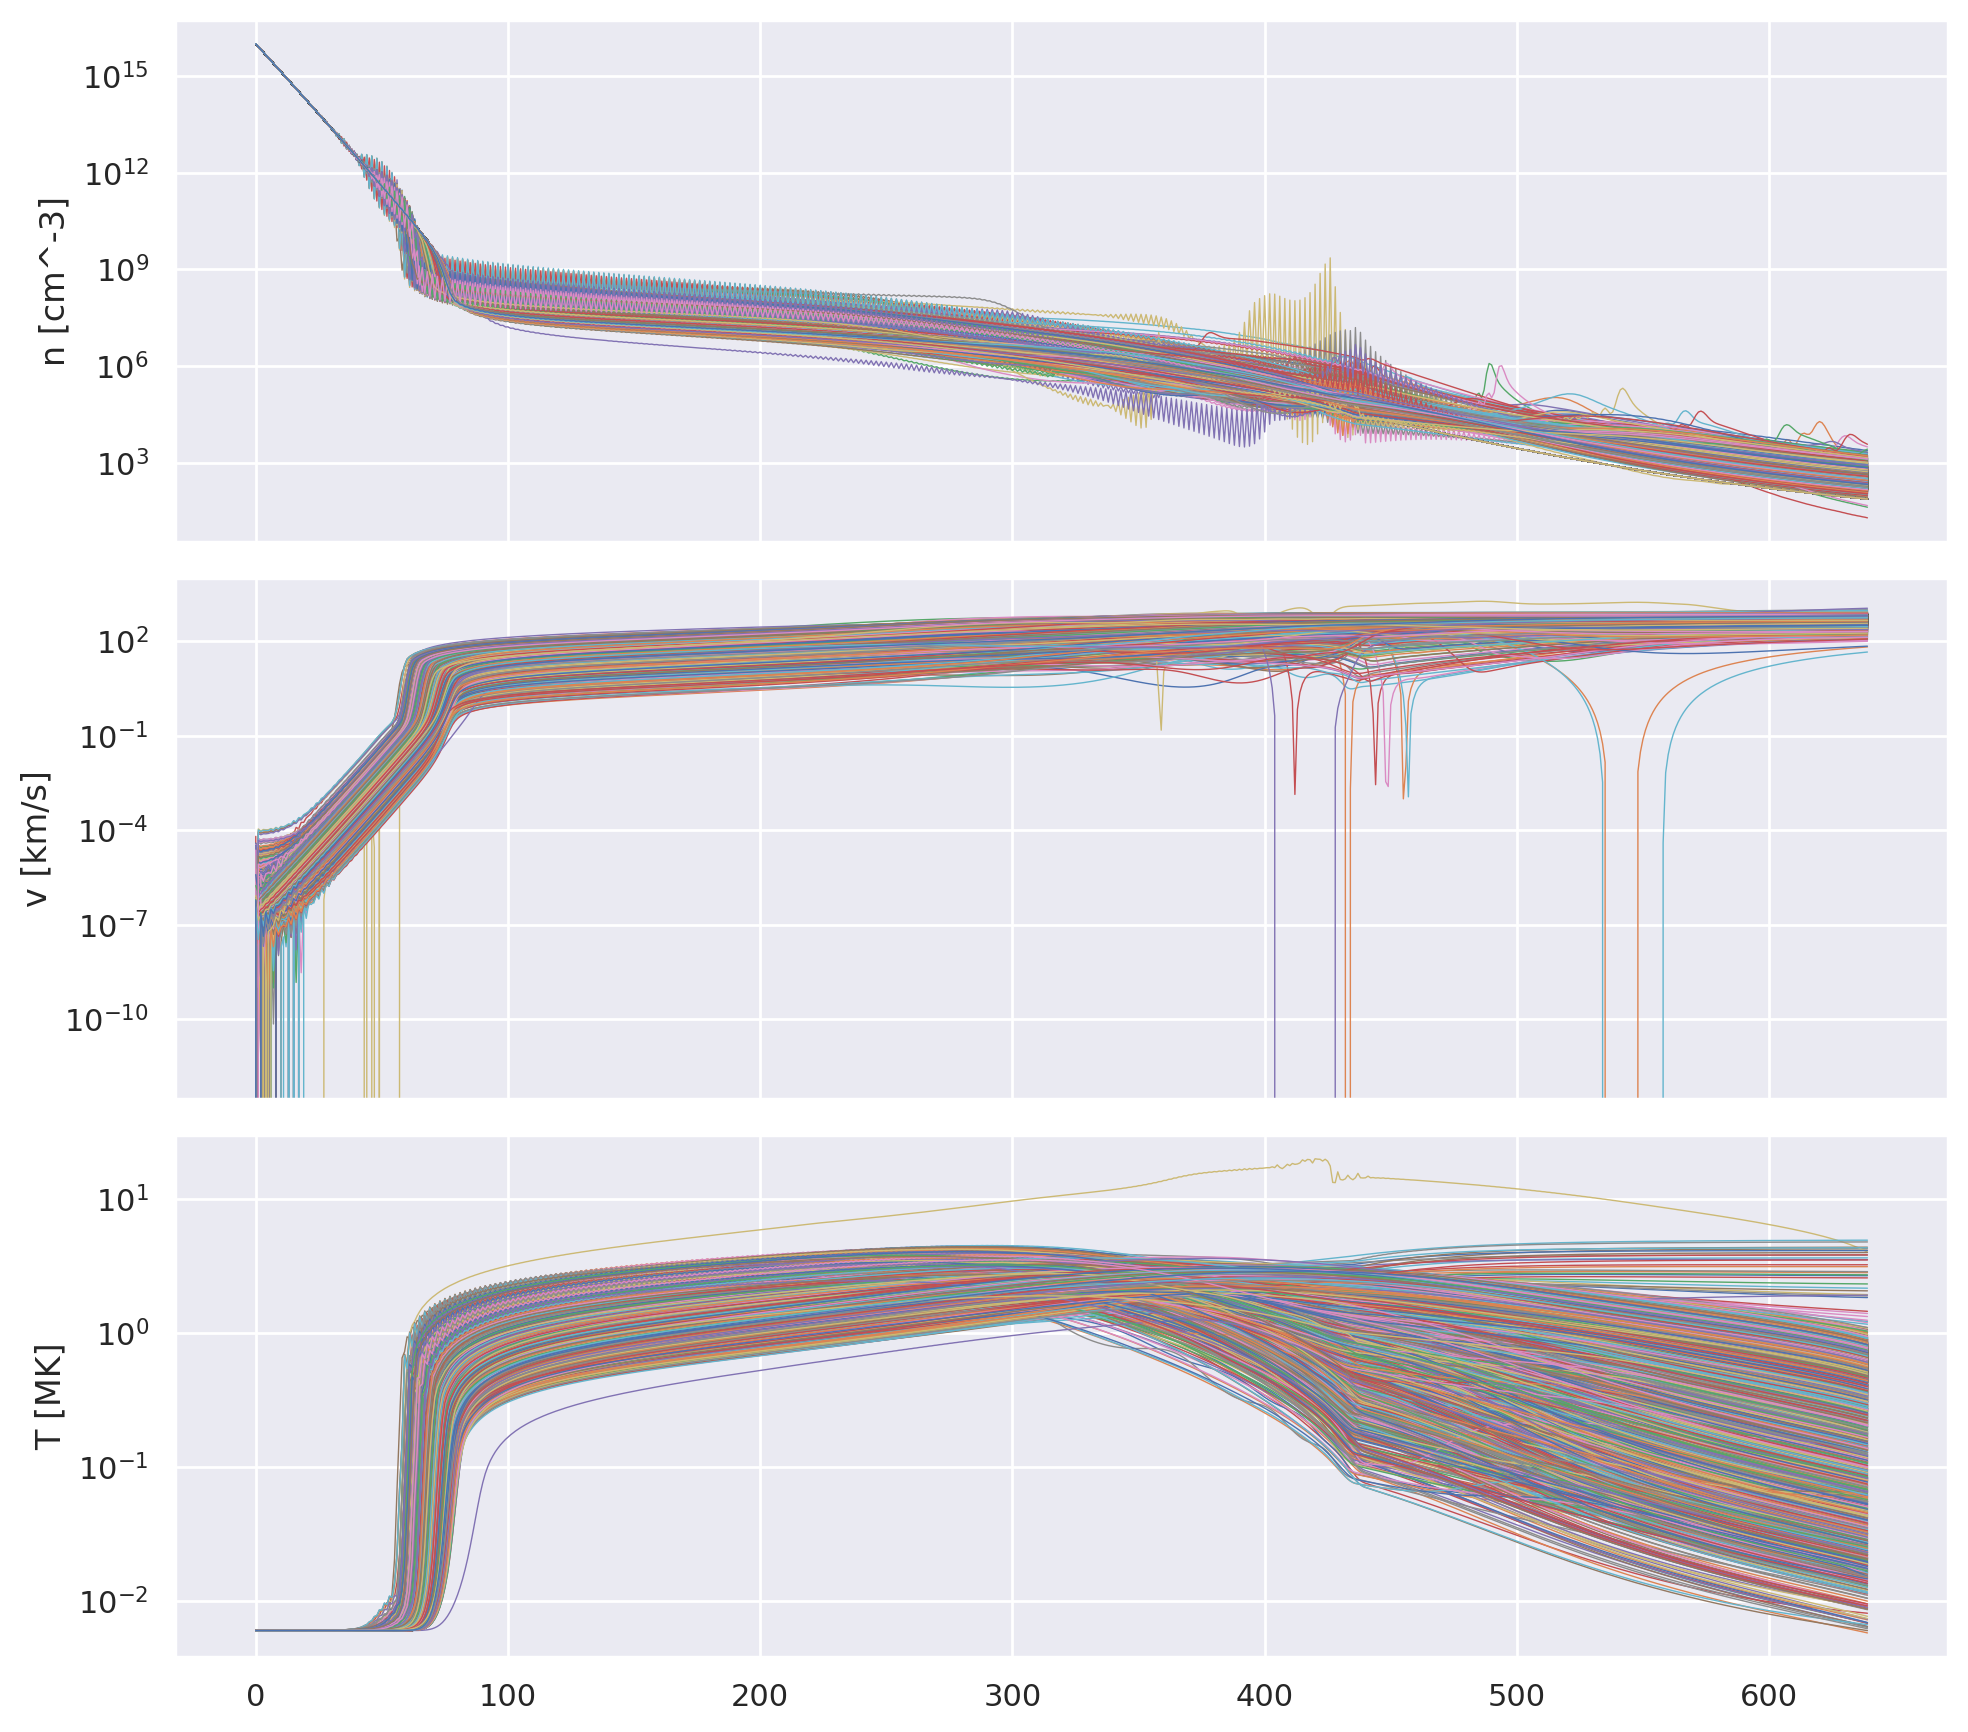
\includegraphics[width=0.8\textwidth]{figures/joint_output_cols.png}
    \caption[Joint plot of the outputs of MULTI-VP]{Joint plot of the output variables of each file used in this work. The first row plots the number of charged particles per unit volume, $n$, the second the velocity, $v$, and the last the temperature, $T$. All are plotted in function of position in the magnetogram file.}
    \label{fig:jointplot_output}
\end{figure}

A preliminary statistical analysis of the data can be seen in tables \ref{tab:data_stats}. The mean, standard deviation, minimum, maximum, and quartiles of each variable are presented in it. Out of the three input columns used, the magnetic field ($B$) has the highest standard deviation, which might indicate that this physical quantity is more prone to anomalies than the others. The radial coordinate ($R$) has the lowest standard deviation, which is expected, as it is almost a constant value for each file. The output variables have a similar standard deviation, with the number of charged particles per unit volume ($n$) having the highest and the temperature ($T$) the lowest. The velocity ($v$) has a standard deviation similar to $T$.

\begin{table}[]
    \caption{Statistical Analysis of the dataset.}
    \label{tab:data_stats}
    \begin{tabular}{@{}lrrrrrr@{}}
    \toprule
           & R {[}Rsun{]} & B {[}G{]} & $\alpha$ {[}deg{]} & $n${[}$cm^{-3}${]} & $v${[}$km/s${]} & $T${[}$MK${]} \\ \midrule
    mean   & 4.755        & 5.471     & 1.885              & 8.630e+13 & 2.553e+02  & 1.384     \\
    std    & 7.165        & 9.178e+01 & 1.472e+01          & 6.839e+14 & 2.148e+02  & 8.968e-01 \\
    min    & 1.000        & 5.122e-05 & -8.763e+01         & 1.973e+01 & -6.757e-03 & 5.765e-03 \\
    $25\%$ & 1.021        & 4.051e-02 & -1.079e-01         & 1.622e+04 & 4.926e+01  & 7.179e-01 \\
    $50\%$ & 1.151        & 2.095     & 0.000              & 2.351e+06 & 2.110e+02  & 1.337     \\
    $75\%$ & 4.250        & 5.582     & 9.997e-01          & 2.132e+07 & 4.508e+02  & 2.098     \\
    max    & 3.150e+01    & 2.470e+05 & 8.925e+01          & 1.010e+16 & 1.889e+03  & 1.990e+01 \\ \bottomrule
    \end{tabular}
    \end{table}


\begin{figure}[h]
    \centering
    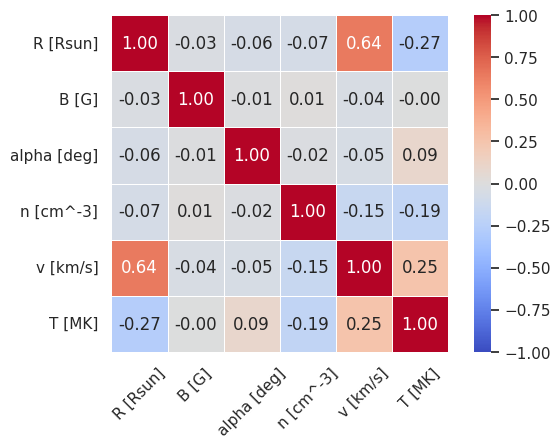
\includegraphics[width=0.8\textwidth]{figures/variables_corrplot.png}
    \caption{Correlation plot of all variables used in this work.}
    \label{fig:corrplot}
\end{figure}

In addition to these statistics, the correlation between the variables can be seen in Figure \ref{fig:corrplot}. There is virtually no correlation between the input variables ($R$, $B$, and $\alpha$), which is expected, as they are independent observations. 

The output variables ($n$, $v$, and $T$) are somewhat correlated. The temperature, $T$, is positively correlated with the velocity of the solar wind, $v$, which is expected as with higher wind speeds, the particles there is a tendency for higher temperatures. The opposite is true for the volume density of the solar wind, $n$, which is negatively correlated with the temperature. This is expected as with higher densities, the particles will have less kinetic energy and, therefore, a lower temperature. The velocity of the solar wind is also slightly negatively correlated with the volume density.

A high correlation between the radial coordinate $R$ and the velocity $v$ can be observed, as $v$ is expected to increase with distance from the Sun. Additionally, the temperature of the solar wind drops as the distance to the Sun increases, which is reflected in the negative correlation between $R$ and $T$.


\begin{figure}
    \centering
    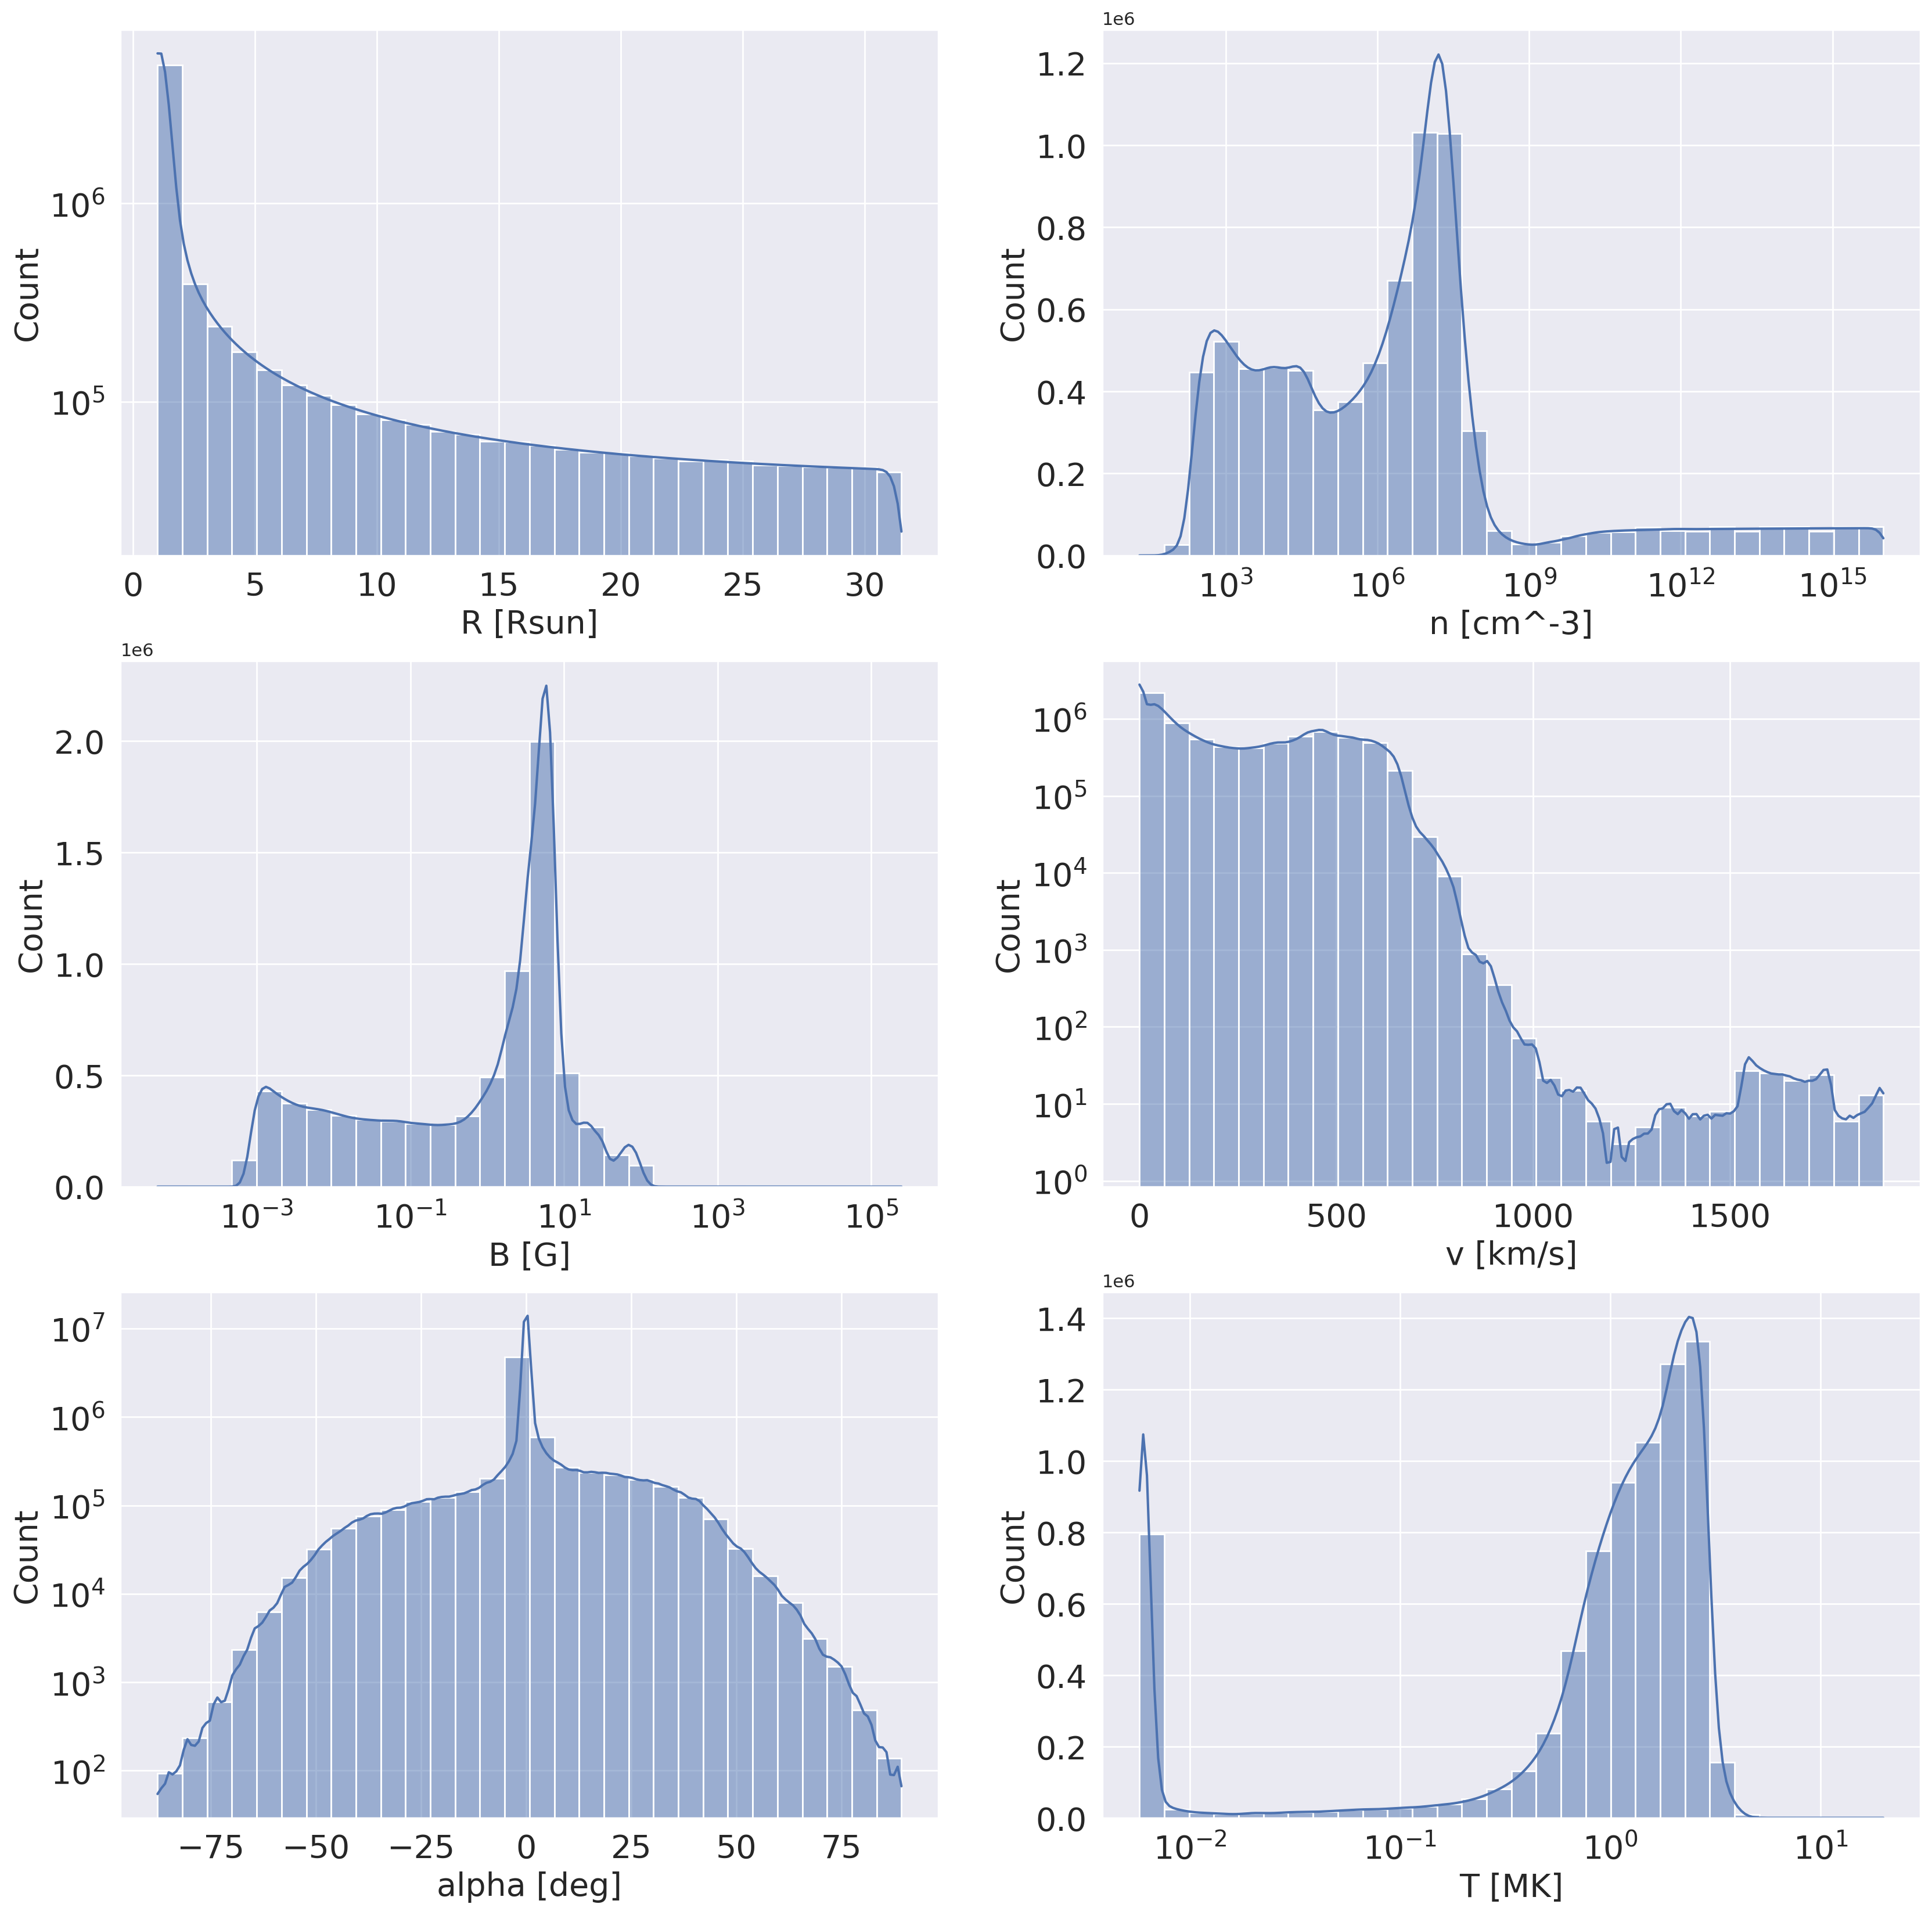
\includegraphics[width=\textwidth]{figures/joint_var_distribution.png}
    \caption[Value distribution of the dataset variables]{Plot of the value distributions of the input (left) and output (right) variables.}
    \label{fig:joint_vars_distr}
\end{figure}

A distribution plot of each input variable can be seen in the left column of Figure \ref{fig:joint_vars_distr}. As expected, the values of $R$ range from 1 to about 31.5. This is corroborated by Table \ref{tab:data_stats}, with most values concentrated around 1. $B [G]$ displays a skewed distribution. At the same time, $\alpha [deg]$ is more evenly distributed (almost symmetric in relation to $x=0$).

Contrary to the findings in the input variables, the values of the output variables are much less evenly distributed. The number of charged particles per unit volume, $n$, has a very skewed distribution, with most values being concentrated in the $10^{3}$ to $10^{7}$ range. The velocity, $v$, has a larger distribution of values, with most indicating slower velocities. The temperature, $T$, has a strange distribution, with most values concentrated near 0 and the rest ranging from 0.5 to 5.

% \clearpage
\section{Hypothesis}\label{sec:hypothesis}
In an attempt to solve the issues of the previous approaches, the following hypothesis can be formulated:
\begin{quote}
    % In conjunction with the preexisting ones, new machine-learning methods can be used for initial condition estimation to improve the quality of these estimates, resulting in a better solution and execution times for the MULTI-VP simulator.
    By integrating clustering and adversarial anomaly detection techniques, the initial conditions predicted by RNNs for the MULTI-VP simulator will be closer to the final simulation results and contribute to faster executions.
    
    % MULTI-VP can achieve better results in a smaller time frame by improving the quality of the previous prediction models for initial conditions with the help of machine learning techniques.
\end{quote}
% \begin{adjustwidth}{2cm}{}
%     GAN-based anomaly detection architectures can accurately and automatically detect outliers in the solar wind profiles data used to train the NN model for initial condition estimation and improve the model's predictions.
% \end{adjustwidth}

The following questions offer a disambiguation of the proposed hypothesis:

\begin{description}
    % \item[Q1] \textit{What do "better" and "improving quality" mean in this context?} These terms apply to MULTI-VP and the initial condition estimation prediction model. They intend to imply that the prediction and simulation model results are closer to the real estimates and more resilient towards noisy data than previous implementations.

    % \item[Q2] \textit{What machine learning techniques will be used for this task?} We intend to use clustering-based techniques to try and find characteristics in the data that would result in better generalizations by the prediction model. In addition to this, we also aim to use adversarial learning methods to detect and filter anomalies in the dataset. With this, the goal is to reduce the effect of the noise input data in the prediction model and make it more resilient to abnormal data.

    \item[Q1] \textit{What do estimates closer to the final simulation mean?} As explained in Section \ref{sec:multivp}, MULTI-VP takes initial flow conditions provided by experts as input and slowly converges to a final and viable solution. With these terms, we intend to verify if the estimates predicted by the RNN models will be nearer to the simulation outputs than the original expert guesses. 

    \item[Q2] \textit{What does "faster execution" mean in this context?} These terms are mainly used to describe the computation time that MULTI-VP takes to reach a viable solution. A faster simulation would mean a decrease in the time the simulation is busy trying to reach a solution. 
\end{description}


Taking these factors into consideration, the research questions of this thesis are:

\begin{description}
    \item[RQ1] \textit{Are clustering methods capable of detecting characteristics in the dataset that were overlooked by the original RNN and would help with the prediction task?}
     This question aims to assess the potential improvement in estimating solar wind by incorporating clustering techniques during the training of the prediction model. Specifically, it investigates whether the clustering methods can identify and capture dataset characteristics previously overlooked by earlier iterations of the RNN model. The objective is to determine if the integration of clustering techniques can ultimately result in better estimates of solar wind.

    \item[RQ2] \textit{Do the estimates obtained with clustering-based training significantly improve the simulation's performance?} This question aims to validate whether using clustering in the method significantly reduces the computation time of MULTI-VP for solar wind estimates. In addition, we are trying to assert if the final estimates from MULTI-VP are closer to the desired outcome.
    
    \item[RQ3] \textit{Can adversarial learning methods detect anomalies in solar wind profiles?} Considering anomaly samples as the positive class, we mostly try to reduce the False Negative Rate (FN) since it has the most detrimental impact on the training of the predictive model. As a secondary priority, we will focus on reducing the amount of False Positives (FP) to ensure that almost no relevant samples are excluded from the training process.
    
    \item[RQ4] \textit{Does the resulting dataset significantly improve the predictive ability of the RNN?} If the resulting dataset following the removal of anomalies leads to an improvement in the model used to predict initial conditions from input flows. In other words, does the mean square distance between the actual estimations and those predicted by the model decrease compared to the previous method?
    \item[RQ5] \textit{Does the improved predictive ability of the RNN result in a further reduction of execution time for MULTI-VP?} This question aims to clarify if the developed model for initial flow estimation can produce improved approximations of solar wind flows and thus reduce the time it takes for MULTI-VP to reach a solution.
\end{description}



\section{Methodology}
To tackle the abovementioned questions, we will employ clustering techniques on the magnetogram data from various sources (e.g., Wilcox Solar Observatory) to improve the performance of the initial flow estimation model. With initial conditions closer to the final ones, we expect that MULTI-VP will reach better solutions in a smaller time frame. The research approach for this phase will be performed quantitatively, with the estimates from this new method being compared to the ones obtained in Barros \cite{barros_InitialConditionEstimation_}.

In addition to this, we will also employ adversarial learning techniques for anomaly detection in solar wind profiles. This approach will be used to assert if extreme data values hinder the RNN model's overall performance and, consequently, the MULTI-VP simulation. The research for this phase will take on a qualitative and quantitative approach. Due to the lack of labelled data and consensus on normal and anomalous profiles, the results from anomaly detection will need to be evaluated visually. In other words, the chosen anomaly detection approach will need to be picked based on the visual inspection of the dataset after anomaly detection. Like in the clustering phase, the comparison of this approach and the previous ones will be made in a quantitive way.















% \section{Methodology}\label{sec:method}
% To evaluate the integrity of the hypothesis, we propose developing a GAN architecture to detect outliers in magnetogram files with an approach similar to the ones in \cite{li.etal_MADGANMultivariateAnomaly_2019}, and \cite{bashar.nayak_TAnoGANTimeSeries_2020}. It will use the generator and the discriminator to detect anomalies in the dataset. 

% The developed anomaly detector will be incorporated into the existing ML methodology expressed in Figure \ref{fig:multivp_rnn}. The resulting representation of the overall data flow for the proposed approach can be seen in Figure \ref{fig:gan_rnn_multivp}. The goal is to use a GAN-based solution to detect outlier samples before training the ML models for initial flow estimation. We propose using the input values of the available magnetograms for this step. The detected anomalies will be removed from the dataset, and the RNN model will be trained with the remaining samples. The new predictions will be compared to the ones from the previous method to evaluate the improvement in the prediction quality. Finally, the predictions will be used as initial conditions for MULTI-VP, and the execution time will be compared to the previous method.

% \begin{figure}[ht]
% \centering
% 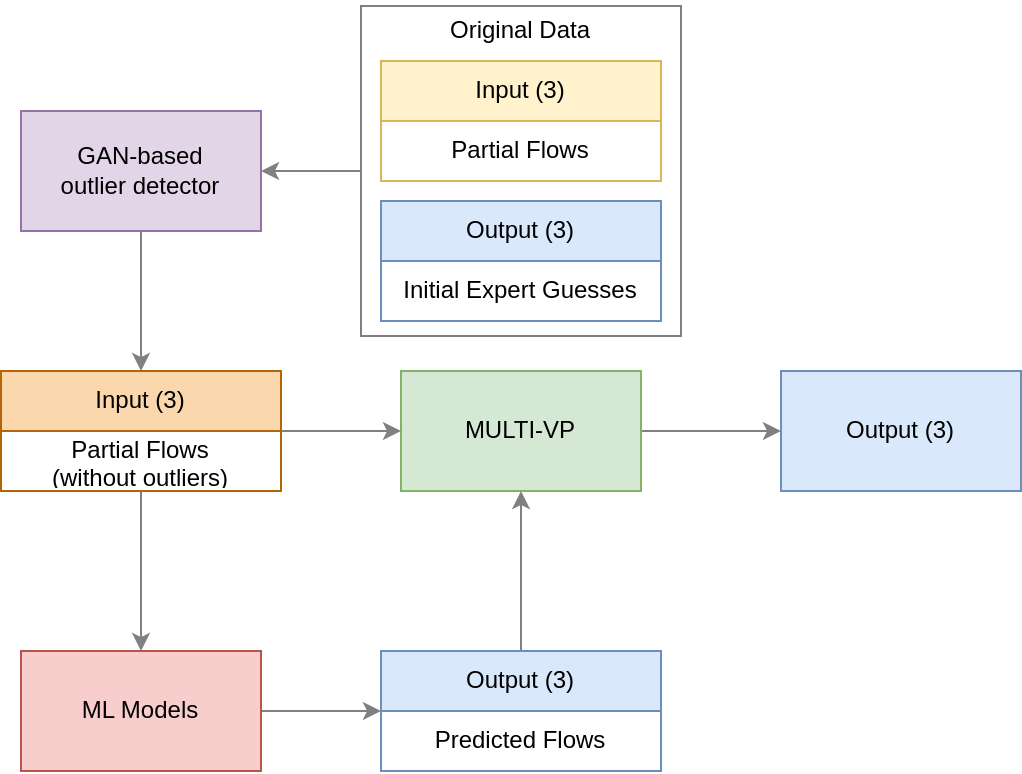
\includegraphics[width=0.8\textwidth]{figures/gan_rnn_multivp.png}
% \caption{GAN-based outlier detection method dataflow.}
% \label{fig:gan_rnn_multivp}
% \end{figure}

% The GAN will have a similar architecture to the one in \cite{goodfellow.etal_GenerativeAdversarialNets_}. During training (Fig. \ref{fig:proposed_gan_train}), the generator's goal is to synthesize magnetogram samples close to the original distribution of the dataset. The discriminator will be tasked with distinguishing fake magnetograms from real ones. %Only normal samples will be used in this process.

% \begin{figure}[ht]
%     \centering
%     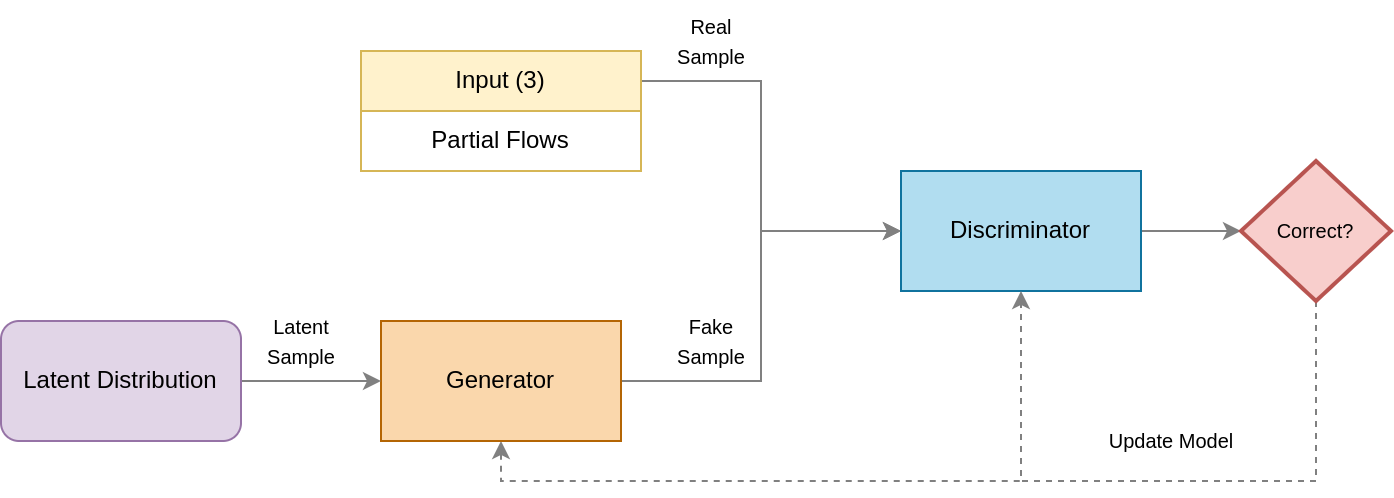
\includegraphics[width=0.8\textwidth]{figures/gan_arch_train.png}
%     \caption{Proposed training method.}
%     \label{fig:proposed_gan_train}
% \end{figure}

% For the detection phase, we propose the methodology in Figure \ref{fig:proposed_gan_arch} with the components trained in the previous stage. First, a sample will be extracted from the dataset and passed directly to the discriminator. If the sample is abnormal, it will most likely have a higher loss than normal ones, as the discriminator only retained the normal data distribution. Next, the sample is mapped into the latent space, where one of the methods from \cite{li.etal_MADGANMultivariateAnomaly_2019} or \cite{bashar.nayak_TAnoGANTimeSeries_2020} could be used. The resulting latent sample is then fed to the generator, which is tasked with reconstructing it. In the next step, the reconstructed sample is compared with the real one, and the reconstruction error is calculated. In theory, if the real sample is defective, then the reconstruction error will be much higher when compared to normal examples, as the generator only learned to generate samples from the normal distribution. In the end, discriminator loss and the reconstruction error will be combined to calculate the anomaly score. The example is considered an anomaly if this score exceeds a predefined threshold.

% \begin{figure}[ht]
% \centering
% 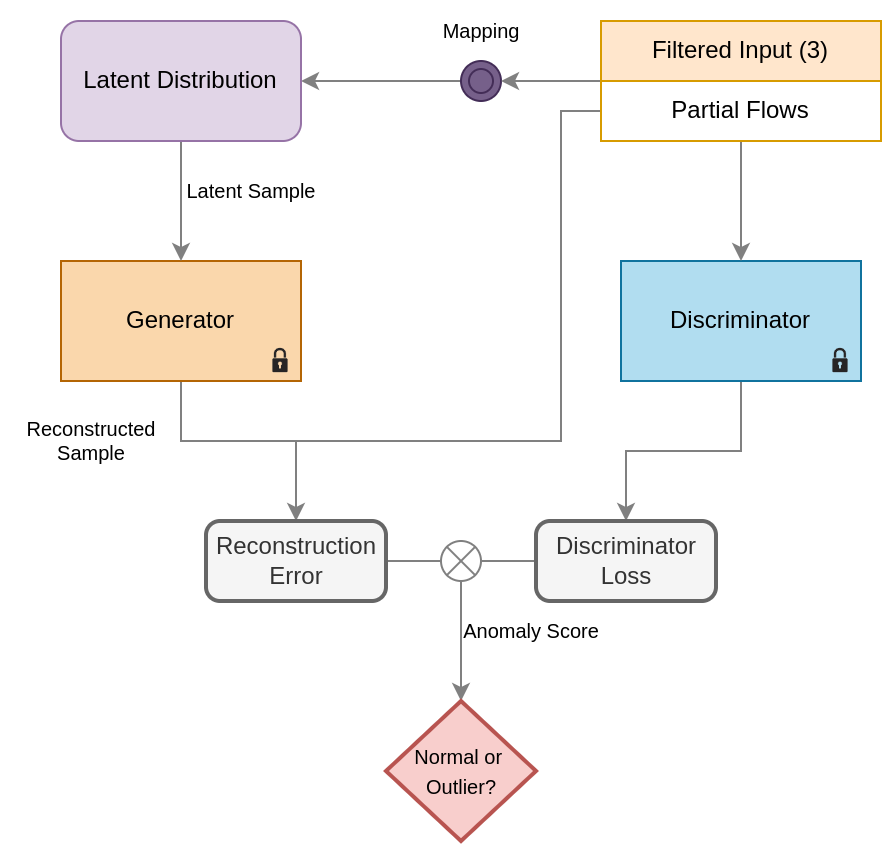
\includegraphics[width=0.8\textwidth]{figures/proposed_gan_arch.png}
% \caption{Proposed method for anomaly detection in magnetogram data.}
% \label{fig:proposed_gan_arch}
% \end{figure}


% The results will be evaluated in an initial step by comparing the distance between the predicted initial estimation of the ML model and the real ones. Similar to the work carried out in \cite{barros_InitialConditionEstimation_}, we will measure the Mean Squared Error (MSE) between the two. Subsequently, the filtered inputs from the outlier detection step will be fed to MULTI-VP along with the initial flow estimations from the ML model. Then the simulation execution times when using the proposed methodology will be compared with the previous implementations to assert if there was a significant reduction.

% \section{Work Plan}\label{sec:work_plan}
% In Figure \ref{fig:work_plan}, an illustration of the proposed work plan is given. In the initial part of development, a more in-depth analysis of the input data will be performed. In addition, we will try to apply some clustering methods to determine if any subgroups in the dataset would facilitate the anomaly detection method.

% In the next stage, a GAN architecture will be designed to detect outliers in magnetogram data. Pytorch \cite{NEURIPS2019_9015} will be the tool used for this goal. Some time was also allocated to implementing GANs with this framework. After developing a suitable method for outlier detection on the given dataset, an extensive analysis of the performance of the ML model with the data without outliers will be done. This part will be used to validate the hypothesis defined in Section \ref{sec:hypothesis}. During this time, some adjustments might have to be made to the initial solution to overcome any shortcomings on these tests. As was already stated, we will use the MSE between the actual estimations and those predicted with the new method. 

% After finetuning, the newly improved estimations from the previous step will be used on MULTI-VP to evaluate if the chosen implementation resulted in a shorter execution time. The final stage will be dedicated to writing the dissertation and accommodating any delays from the previous steps.

% \begin{figure}[ht]
% \centering
% 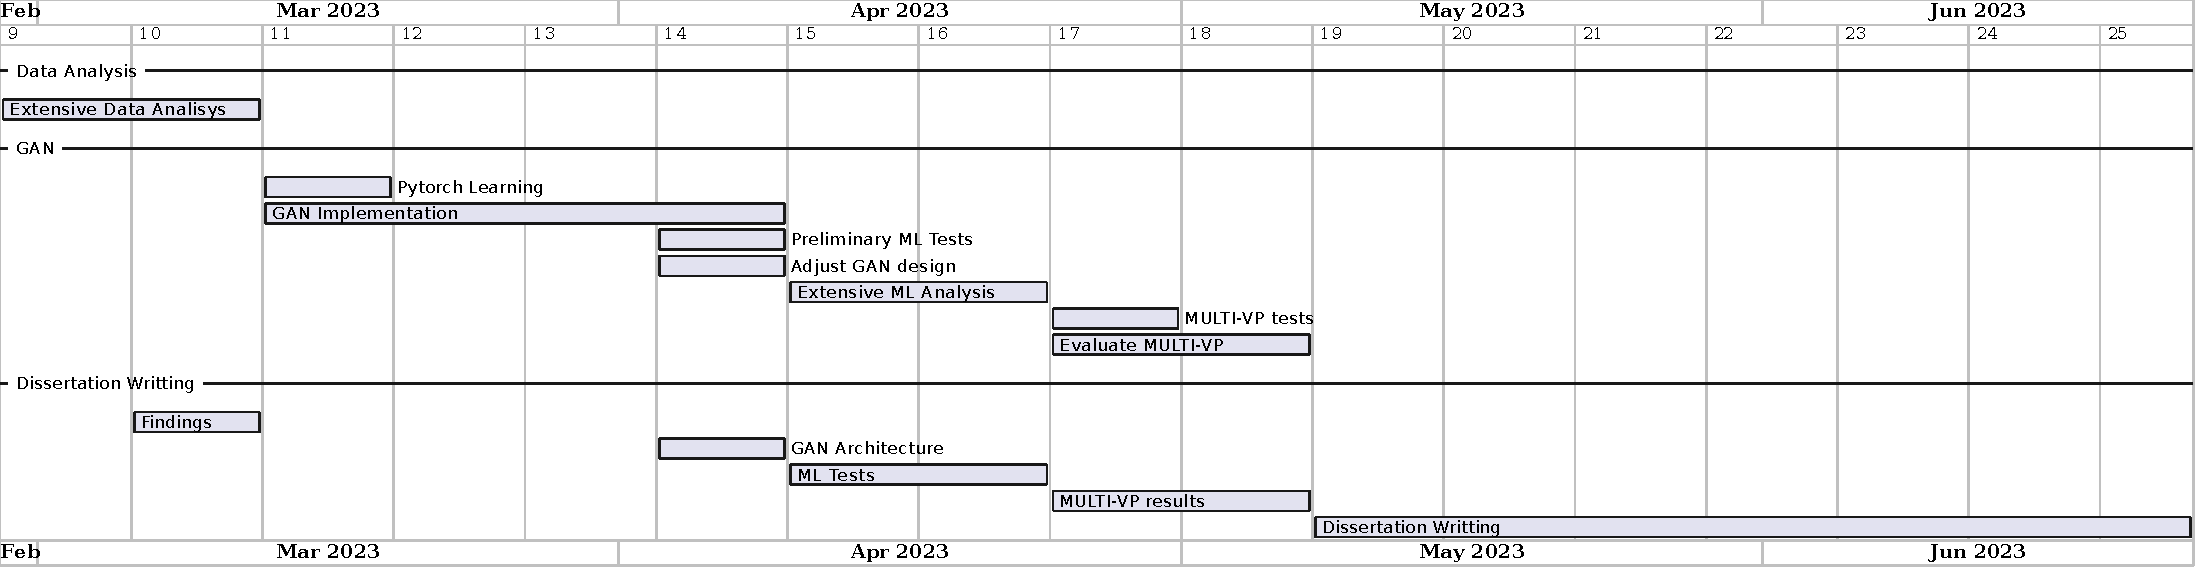
\includegraphics[width=\textwidth]{figures/work_plan.pdf}
% \caption{Proposed development plan.}
% \label{fig:work_plan}
% \end{figure}
